\chapter{Sample-efficient Q-Learning in SMDPs}
\label{Chapter4}

The effects of using temporal abstraction are then difficult to predict. In this section, we will study the sample efficiency of the algorithm for SMDP presented in the previous chapter \ref{subsec:SMDP}, Q-Learning. More specifically, we shall adapt the latest and tightest sample complexity result in the literature for classical QL to the SMDP case. This kind of theoretical guarantees for such basic SMDP algorithm is still lacking in the literature, and it could be interesting to see the change with temporally extended actions.

\section{Sample complexity of Q-Learning}
\label{sec:SC-QL}

First of all, we shall go through the results and the outlines of the proof from the paper \citep{li_sample_2021}. Hence \textbf{a lot of the following content is directly taken from this paper}.

The paper focuses on asynchronous QL as described in section \ref{subsec:Rl-QL}, where the goal is to learn $Q^*$ from a history $\left( s_t, a_t, r_t \right)_{t=0}^\infty$ generated under behaviour policy $\pi_b$. In particular, this works aims to provide a (tight) minimum time step $T$ such that
\begin{align}
  \|\mathbf{Q}_T - \mathbf{Q}^*\|_\infty = \max_{(s,a) \in \mathcal{S}\times \mathcal{A}} |Q_T(s,a) - Q^*(s,a)| \leq \epsilon \label{SC-def}
\end{align}
with probability $1-\delta$, for some user-defined parameters $\delta$ and $\epsilon$, where $\mathbf{Q}_T$ is the Q-value matrix estimate at time $T$.

Before presenting the result and going into the details of the proof, some notations must be introduced.

\subsection{Notations and assumptions}
\label{subsec:notations}

In the following, letters in bold like $\mathbf{Q}$ shall stand for matrices and vectors, and for a matrix $\mathbf{M} \in \mathbb{R}^{N\times L}$, $\mathbf{M(i)}$ is the $i$-th row of $\mathbf{M}$. Also, as long as there is no confusion, applying operations such as $\sqrt{\cdot}$ or $|\cdot|$ to a matrix is the entry-wise operation: $|\mathbf{M}| = (|m_{ij}|)_{i,j}$. Finally, $\mathbf{1}$ is the vector full of ones and $\mathbf{I}$ is the identity matrix.

As said in the chapter \ref{chapter2}, the behaviour policy $\pi_b$ induces a Markov Chain. It is assumed that this Markov Chain is \emph{uniformly ergodic}, where we remind the definition of ergodicity in \ref{ergodicity}. This ensures that all states are visited infinitely often and the Chain converges to its stationary regime at a geometric pace. More specifically, it allows for the definition of the following parameters:

\begin{align}
  &\mu_{min} = \min_{(s,a) \in \mathcal{S}\times \mathcal{A}} \mu (s,a)\\
  &t_{mix} = \min \left\{ t \,|\, \max_{(s_0,a_0) \in \mathcal{S}\times \mathcal{A}} d_{TV}(P^t(\cdot \,|\, s_0, a_0), \mu) \leq \frac{1}{4} \right\}\\
  &t_{cover} = \min \left\{ t \,|\, \min_{(s_0,a_0) \in \mathcal{S}\times \mathcal{A}} \mathbb{P} \left(\mathcal{B}_t \,|\, s_0, a_0 \right) \geq \frac{1}{2} \right\}\\
  &t_{frame} = \frac{443 t_{mix}}{\mu_{min}}\log\left( \frac{4SA}{\delta} \right)\\
  &t_{th} = \max \left\{ \frac{2 \log\left( \frac{1}{(1-\gamma)^2 \epsilon} \right) }{\eta \mu_{min}}, t_{frame} \right\}\label{eq:t_th}\\
  &\rho = (1-\gamma)(1 - (1 - \eta)^{\mu_{frame}}) \label{eq:rho}
\end{align}

where $\mu$ is the stationary distribution of the Markov Chain, $d_{TV}$ is the total variation distance between distributions and $\mathcal{B}_t$ is the event that all state-action pairs have been visited at least once before time step $t$. $\mu_{min}$ is the smallest probability density for a state-action pair, $t_{mix}$ represents the time needed to be remove the influence of the initial state, and $t_{cover}$ gives an order of magnitude of the time needed to visit all the state-action space. The three over quantities appear naturally as the proof goes.

In order to analyse the QL update in a matrix-form way, we introduce
\begin{align}
  \mathbf{\Lambda}_t ((s,a), (s,a)) = \begin{cases} \eta & \text{if }(s,a) = (s_{t-1}, a_{t-1})\\ 0 & \text{otherwise}\end{cases}\\
  \mathbf{P}_t((s,a), s') = \begin{cases}1 &\text{if } (s,a,s') = (s_{t-1}, a_{t-1}, s_t)\\ 0 & \text{otherwise}\end{cases}
\end{align}

and we will use $\mathbf{Q}_t$ for the Q-value matrix, $\mathbf{P}$ for the transition matrix and $\tilde{\mathbf{P}}$ for the expected discounted probability matrix (cf \ref{thm:values-SMDP}). Notice that $\mathbf{\Lambda}_t \in [0,1)^{SA \times SA}$ is diagonal, and $\mathbf{P}_t \in [0,1]^{SA \times S}$. Then we have, for the classical setting and for SMDP respectively:
\begin{align}
  \mathbf{Q}_t = (\mathbf{I} - \mathbf{\Lambda}_t)\mathbf{Q}_{t-1} + \mathbf{\Lambda}_t (\mathbf{r} + \gamma \mathbf{P}_t \mathbf{V}_{t-1})\label{eq:QL-update}\\
  \tilde{\mathbf{Q}}_t = (\mathbf{I} - \mathbf{\Lambda}_t)\tilde{\mathbf{Q}}_t + \mathbf{\Lambda}_t (\mathbf{r} + \tilde{\mathbf{P}}_t \tilde{\mathbf{V}}_{t-1})\label{eq:SQL-update}
\end{align}

Finally, we will be interested in the following quantity:

\begin{align}
  \mathbf{\Delta}_t = \mathbf{Q}_t - \mathbf{Q}^*\label{eq:Delta}
\end{align}


\subsection{Main result and proof}
\label{subsec:thm1}

The main result is presented in the following theorem:

\begin{thm}[Sample complexity of AQL]\label{thm:1}
  There exists universal constants $c_0, c_1 > 0$ such that for any $\delta \in (0,1)$, $\epsilon \in (0, \frac{1}{1 - \gamma}]$, (\ref{SC-def}) holds with probability $1 - \delta$ for
    \begin{align}
      T \geq \frac{c_0}{\mu_{min}} \left\{ \frac{1}{(1 - \gamma)^5\epsilon^2} + \frac{t_{mix}}{1 - \gamma} \right\}\log\left(\frac{SA}{\delta}\right)\log\left(\frac{1}{(1-\gamma)^2 \epsilon}\right)\label{eq:T}\\
      \eta = \frac{c_1}{\log(\frac{SAT}{\delta})} \min \left\{ \frac{(1-\gamma)^4 \epsilon^2}{\gamma^2}, \frac{1}{t_{mix}} \right\}\label{eq:eta}
    \end{align}
\end{thm}
where $\eta = \alpha_t$ is the constant learning rate used. By \emph{universal constant} is meant a constant that does not depend on $\epsilon, \delta, t, \eta$ nor another parameter of the MDP.

The main step in the proof is the Theorem \ref{thm:5}:

\begin{thm}[Theorem 5]\label{thm:5}
  For any $\epsilon \in (0, \frac{1}{1-\gamma}]$, $\delta \in (0, 1)$, there exists a universal constant $c > 0$ such that with probability at least $1 - 6\delta$, for all $t \leq T$:
    \begin{align}
      \|\mathbf{Q}_t - \mathbf{Q}^*\|_\infty \leq (1-\rho)^k \frac{\|\mathbf{Q}_0 - \mathbf{Q}^*\|_\infty}{1-\gamma} + \frac{c \gamma}{1-\gamma}\|\mathbf{V}^*\|_\infty \sqrt{\eta \log\left( \frac{SAT}{\delta} \right)} + \epsilon \label{eq:thm5}
    \end{align}
    with $k = \max \left\{ 0, \lfloor \frac{t - t_{th}}{t_{frame}} \rfloor \right\}$.
\end{thm}

It is easy to upper-bound the second term of (\ref{eq:thm5}) with $\epsilon$ by defining $\eta$ as in (\ref{eq:eta}). Then, two inequalities
\begin{align}
  &(1-\rho)^k \frac{\|\mathbf{\Delta}_0\|_\infty }{1-\gamma} \leq e^{- \rho k}\frac{\left\| \mathbf{\Delta}_0 \right\|_\infty}{1-\gamma}\\
  &\rho \geq \frac{1}{2}(1-\gamma)\eta\mu_{frame} \quad \text{ when } \eta < \frac{1}{\mu_{frame}}
\end{align}
can be applied on the first term to then upper-bound the latter with $\epsilon$ thanks to the definition of $k$, as long as
\begin{align}
  &t \geq t_{th} + t_{frame} + \frac{4}{(1-\gamma)\eta \mu_{min}} \log\left( \frac{\left\| \mathbf{\Delta}_0 \right\|_\infty}{\epsilon(1-\gamma)} \right) = T
\end{align}

Now, to prove Theorem \ref{thm:5}, the first stepping stone is the following recursive decomposition, based on the matricial form of the QL-update and property of $Q^*$ being a fixed point of the optimal Bellman operator ($\mathbf{Q}^* = \mathbf{r} + \gamma \mathbf{P}\mathbf{V}^*$):

\begin{align}
  \mathbf{\Delta}_t &= (\mathbf{I}-\mathbf{\Lambda}_t)\mathbf{Q}_{t-1} + \mathbf{\Lambda}_t(\mathbf{r} + \gamma \mathbf{P}_t \mathbf{V}_{t-1}) - \mathbf{Q}^*\label{eq:1}\\
  &= (\mathbf{I}-\mathbf{\Lambda}_t)(\mathbf{Q}_{t-1} - \mathbf{Q}^*) + \mathbf{\Lambda}_t(\mathbf{r} + \gamma \mathbf{P}_t \mathbf{V}_{t-1} - \mathbf{Q}^*)\label{eq:2}\\
  &= (\mathbf{I}-\mathbf{\Lambda}_t)(\mathbf{Q}_{t-1} - \mathbf{Q}^*) + \gamma\mathbf{\Lambda}_t(\mathbf{P}_t \mathbf{V}_{t-1} - \mathbf{P}\mathbf{V}^*)\label{eq:3}\\
  &= (\mathbf{I}-\mathbf{\Lambda}_t)\mathbf{\Delta}_t + \gamma\mathbf{\Lambda}_t(\mathbf{P}_t - \mathbf{P}) \mathbf{V}^* + \gamma \mathbf{\Lambda}_t\mathbf{P}_t (\mathbf{V}_{t-1} - \mathbf{V}^*)\label{eq:4}
\end{align}

By induction, one can see that we get

\begin{align}
  \mathbf{\Delta}_t = \underbrace{\gamma\sum_{i=1}^{t}\prod_{j=i+1}^{t}(\mathbf{I}-\mathbf{\Lambda}_j)\mathbf{\Lambda}_i (\mathbf{P}_i - \mathbf{P})\mathbf{V}^*}_{\beta_{1,t}} + \underbrace{\gamma \sum_{i=1}^{t}\prod_{j=i+1}^{t}(\mathbf{I}-\mathbf{\Lambda}_j)\mathbf{\Lambda}_i \mathbf{P}_i (\mathbf{V}_{i-1} - \mathbf{V}^*)}_{\beta_{2,t}} + \underbrace{\prod_{j=1}^{t}(\mathbf{I}-\mathbf{\Lambda}_j)\mathbf{\Delta}_0}_{\beta_{3,t}} \label{eq:betas}
\end{align}

hence
\begin{align}
  \left| \mathbf{\Delta}_t \right| \leq \left| \beta_{1,t} \right| + \left| \beta_{2,t} \right| + \left| \beta_{3,t} \right|\label{eq:betas2}
\end{align}

where $\leq$ means that the inequality holds for all entries of the matrices. The next step is to upper-bound each of these three part of the decomposition.

First off with a simple upper-bounding of $\beta_{2,t}$:

\begin{align}
  &\left\| \mathbf{P}_i(\mathbf{V}_{i-1} - \mathbf{V}^*) \right\|_\infty \leq \left\| \mathbf{P}_i \right\|_1 \left\| \mathbf{V}_{i-1} - \mathbf{V}^* \right\|_\infty = \left\| \mathbf{Q}_{i-1} - \mathbf{Q}^* \right\|_\infty = \left\| \mathbf{\Delta}_{i-1} \right\|_\infty\\
  &\implies \left| \beta_{2,t} \right| \leq \gamma \sum_{i=1}^{t} \left\| \mathbf{\Delta}_{i-1} \right\|_\infty \prod_{j=i+1}^{t}(\mathbf{I}-\mathbf{\Lambda}_j)\mathbf{\Lambda}_i \mathbf{1}\label{eq:beta2}
\end{align}

Then, for $\beta_{1,t}$:
\begin{lem}[Lemma 1]\label{lem:1}
  There exists a universal constant $c >0$ such that, for any $0<\delta<1$:
  \begin{align}
    \forall \, 1\leq t \leq T,\quad \left| \gamma \sum_{i=1}^{t}\prod_{j=i+1}^{t}(\mathbf{I}-\mathbf{\Lambda}_j)\mathbf{\Lambda}_i (\mathbf{P}_i-\mathbf{P})\mathbf{V}^* \right| \leq \tau_1 \left\| \mathbf{V}^* \right\|_\infty \mathbf{1} \label{eq:lem1}
  \end{align}
  with probability $1-\delta$, and $\tau_1 = c\gamma \sqrt{\eta \log\left( \frac{SAT}{\delta} \right)}$.
\end{lem}
The proof for this lemma relies on the fact that $(\mathbf{P}_i - \mathbf{P})$ concentrates around 0.

Lastly, a result based on the properties of the Markov Chain:

\begin{lem}[Lemma 2]\label{lem:2}
  \begin{align}
    \forall \, t,\quad \left| \prod_{j=1}^{t}(\mathbf{I}-\mathbf{\Lambda}_j)\mathbf{\Delta}_0 \right| \leq \left\| \mathbf{\Delta}_0 \right\|_\infty \mathbf{1}\label{eq:lem2-1}
  \end{align}
  And with probability $1-\delta$, assuming $T > t_{frame}$:
  \begin{align}
    \forall \, t_{frame} \leq t \leq T,\quad \left| \prod_{j=1}^{t}(\mathbf{I}-\mathbf{\Lambda}_j)\mathbf{\Delta}_0 \right| \leq (1-\eta)^{\frac{1}{2}t \mu_{min}} \left| \mathbf{\Delta}_0 \right| \leq (1-\eta)^{\frac{1}{2}t \mu_{min}} \left\| \mathbf{\Delta}_0 \right\|_\infty \mathbf{1} \label{eq:lem2-2}
  \end{align}
\end{lem}

From those upper-bounds, (\ref{eq:beta2}) can be reworked as

\begin{align}
  \left| \mathbf{\Delta}_t \right| \leq \begin{cases} \gamma \sum_{i=1}^{t}\left\| \mathbf{\Delta}_{i-1} \right\|_\infty \prod_{j=i+1}^{t} (\mathbf{I}-\mathbf{\Lambda}_j)\mathbf{\Lambda}_i \mathbf{1} + \tau_1 \left\| \mathbf{V}^* \right\|_\infty \mathbf{1} + \left\| \mathbf{\Delta}_0 \right\|_\infty \mathbf{1} & t < t_{frame}\\ \gamma \sum_{i=1}^{t}\left\| \mathbf{\Delta}_{i-1} \right\|_\infty \prod_{j=i+1}^{t} (\mathbf{I}-\mathbf{\Lambda}_j)\mathbf{\Lambda}_i \mathbf{1} + \tau_1 \left\| \mathbf{V}^* \right\|_\infty \mathbf{1} + (1-\eta)^{\frac{1}{2}t \mu_{min}} \left\| \mathbf{\Delta}_0 \right\|_\infty \mathbf{1} & t_{frame} \leq t \leq T\end{cases}\label{eq:delta-UB}
\end{align}

with probability $1 - 2\delta$. The successive application of the following two lemmas finally finishes the proof for Theorem \ref{thm:5}.

\begin{lem}[Lemma 3]\label{lem:3}
  Let
  \begin{align}
    &u_0 = \frac{\left\| \mathbf{\Delta}_0 \right\|_\infty}{1-\gamma}, \quad u_t = \left\| \mathbf{v}_t \right\|_\infty\\
    &\mathbf{v}_t = \begin{cases}\gamma \sum_{i=1}^{t}\prod_{j=i+1}^{t}(\mathbf{I}-\mathbf{\Lambda}_j)\mathbf{\Lambda}_i \mathbf{1}u_{i-1} + \left\| \mathbf{\Delta}_0 \right\|_\infty \mathbf{1} & 1 \leq t \leq t_{th}\\ \gamma \sum_{i=1}^{t}\prod_{j=i+1}^{t}(\mathbf{I}-\mathbf{\Lambda}_j)\mathbf{\Lambda}_i \mathbf{1}u_{i-1} & t >t_{th} \end{cases}
  \end{align}
  then with probability $1 - 2\delta$
  \begin{align}
    \left\| \mathbf{\Delta}_t \right\|_\infty \leq \frac{\tau_1 \left\| \mathbf{V}^* \right\|_\infty}{1-\gamma} + u_t + \epsilon
  \end{align}
\end{lem}

This lemma is the consequence of a direct computational induction from (\ref{eq:delta-UB}), using the fact that $(1-\eta)^{\frac{1}{2}t \mu_{min}} \leq (1 - \gamma)\epsilon$ when $t \geq t_{th}$, and $\left\| \mathbf{\Delta}_0 \right\|_\infty = \left\| \mathbf{Q}^* \right\|_\infty \leq \frac{1}{1-\gamma}$.

\begin{lem}[Lemma 4]\label{lem:4}
  Let
  \begin{align}
    w_k = (1 - \rho)^k \frac{\left\| \mathbf{\Delta}_0 \right\|_\infty}{1-\gamma}
  \end{align}
  for all $k\in \mathbb{N}$. Then, with probability $1 - 2\delta$:
  \begin{align}
    u_t \leq w_{k_t} \quad \text{with } k_t = \max \left\{ 0, \lfloor \frac{t - t_{th}}{t_{frame}} \rfloor \right\}
  \end{align}
\end{lem}

The proof for Lemma \ref{lem:4} relies once again on computational arguments and an induction, and Lemma 8 which is a result aboout the Markov Chain of the problem.

\section{Sample complexity of Q-learning for SMDPs}

Now we can rework the previous elements of proof for \emph{Q-Learning for SMDP}, of which we recall the update:
\begin{align}
  \tilde Q_t(s_{t-1}, a_{t-1}) = (1 - \tilde\eta)\tilde Q_{t-1}(s_{t-1}, a_{t-1}) + \tilde\eta \left(r(s_{t-1}, a_{t-1}) + \gamma^{\tau_{t-1}} \max_{a\in \mathcal{A}} \tilde Q_{t-1} (s_t, a)\right) \label{eq:SQL}
\end{align}

An other important point to remember is that the Markov Chain is the same for MDP or SMDP, thus the corresponding results still hold (in particular Lemma 8 from \cite{li_sample_2021}).

For convenience, let's denote $\gamma_t = \gamma^{\tau_{t-1}}$. The variables that will change shall be marked by a tilde $\sim$, and the new definitions (when not obvious) will be precised at the relevant times of the proof. Last but not least, have in mind that $1 > \gamma^{\tau_{min}} \geq \gamma^\tau$.

\smallskip

Jumping into the adaptation of the proof now, we shall rewrite or point out the differences due to the change in settings. To begin with, because of the difference in the update, the decomposition of $\mathbf{\Delta}_t$ in (\ref{eq:1}) then gives:

\begin{align}
  \tilde{\mathbf{\Delta}}_t &= (\mathbf{I} - \tilde{\mathbf{\Lambda}}_t)\tilde{\mathbf{Q}}_{t-1} + \tilde{\mathbf{\Lambda}}_t(\mathbf{r} + \gamma_t \mathbf{P}_t\tilde{\mathbf{V}}_{t-1}) - \mathbf{Q}^* \label{eq:1b}\\
  &= (\mathbf{I}-\tilde{\mathbf{\Lambda}}_t)(\tilde{\mathbf{Q}}_{t-1} - \mathbf{Q}^*) + \tilde{\mathbf{\Lambda}}_t(\mathbf{r} + \gamma_t\mathbf{P}_t\tilde{\mathbf{V}}_{t-1} - \mathbf{Q}^*)\label{eq:2b}\\
  &= (\mathbf{I}-\tilde{\mathbf{\Lambda}}_t)(\tilde{\mathbf{Q}}_{t-1} - \mathbf{Q}^*) + \tilde{\mathbf{\Lambda}}_t(\gamma_t\mathbf{P}_t\tilde{\mathbf{V}}_{t-1} - \tilde{\mathbf{P}}\mathbf{V}^*) \label{eq:3b}\\
  &= (\mathbf{I}-\tilde{\mathbf{\Lambda}}_t)(\tilde{\mathbf{Q}}_{t-1} - \mathbf{Q}^*) + \tilde{\mathbf{\Lambda}}_t(\gamma_t\mathbf{P}_t - \tilde{\mathbf{P}})\mathbf{V}^* + \gamma_t\tilde{\mathbf{\Lambda}}_t \mathbf{P}_t(\tilde{\mathbf{V}}_{t-1} - \mathbf{V}^*) \label{eq:4b}
\end{align}

with $\mathbf{Q}^* = \mathbf{r} + \tilde{\mathbf{P}}\mathbf{V}^*$. The two noticeable differences with (\ref{eq:4}) are $\gamma$ exchanged with $\gamma_t$ and attached to $\mathbf{P}_t$, and the use of $\tilde{\mathbf{P}}$ instead of $\gamma \mathbf{P}$. Then, a decomposition by induction similar to (\ref{eq:betas}) yields:

\begin{align}
  \tilde{\mathbf{\Delta}}_t = \underbrace{\sum_{i=1}^{t}\prod_{j=i+1}^{t}(\mathbf{I}-\tilde{\mathbf{\Lambda}}_j)\tilde{\mathbf{\Lambda}}_i (\gamma_i \mathbf{P}_i - \tilde{\mathbf{P}})\mathbf{V}^*}_{\tilde\beta_{1,t}} + \underbrace{\sum_{i=1}^{t}\prod_{j=i+1}^{t}(\mathbf{I}-\tilde{\mathbf{\Lambda}}_j)\tilde{\mathbf{\Lambda}}_i \gamma_i \mathbf{P}_i (\tilde{\mathbf{V}}_{i-1} - \mathbf{V}^*)}_{\tilde\beta_{2,t}} + \underbrace{\prod_{j=1}^{t}(\mathbf{I}-\tilde{\mathbf{\Lambda}}_j)\tilde{\mathbf{\Delta}}_0}_{\tilde\beta_{3,t}} \label{eq:betas-b}
\end{align}

First of all, $\tilde\beta_{3,t} = \beta_{3,t}$ (the difference between $\left\| \tilde{\mathbf{\Delta}}_0 \right\|_\infty$ and $\left\| \mathbf{\Delta}_0 \right\|_\infty$ doesn't matter), so Lemma \ref{lem:2} holds for SMDP. Then, it is easy to go from (\ref{eq:beta2}) to
\begin{align}
  \left| \tilde\beta_{2,t} \right| \leq \gamma^{\tau_{min}} \sum_{i=1}^{t}\left\| \tilde{\mathbf{\Delta}}_{i-1} \right\|_\infty \prod_{j=i+1}^{t}(\mathbf{I}-\tilde{\mathbf{\Lambda}}_j)\tilde{\mathbf{\Lambda}}_i \mathbf{1}
\end{align}

However, a bit of work is needed to prove the following adaptation of Lemma \ref{lem:1}: the proof is deferred to the Appendix \ref{AppendixA}.

\begin{lem}[Lemma 1 bis] \label{lem:1b}
  There exists a universal constant $c >0$ such that, for any $0<\delta<1$:
  \begin{align}
    \forall \, 1\leq t \leq \tilde T,\quad \left| \sum_{i=1}^{t}\prod_{j=i+1}^{t}(\mathbf{I}-\tilde{\mathbf{\Lambda}}_j)\tilde{\mathbf{\Lambda}}_i (\gamma_i \mathbf{P}_i-\tilde{\mathbf{P}})\mathbf{V}^* \right| \leq \tilde\tau_1 \left\| \mathbf{V}^* \right\|_\infty \mathbf{1} \label{eq:lem1}
  \end{align}
  with probability $1-\delta$, and $\tilde\tau_1 = c \gamma^{\tau_{min}} \sqrt{\tilde\eta \log\left( \frac{SA\tilde T}{\delta} \right)}$.
\end{lem}

Finally, the adapted decomposition for SMDP is, with probability $1-2\delta$:

\begin{align}
  \left| \tilde{\mathbf{\Delta}}_t \right| \leq \begin{cases} \gamma^{\tau_{min}} \sum_{i=1}^{t}\left\| \tilde{\mathbf{\Delta}}_{i-1} \right\|_\infty \prod_{j=i+1}^{t} (\mathbf{I}-\tilde{\mathbf{\Lambda}}_j)\tilde{\mathbf{\Lambda}}_i \mathbf{1} + \tilde\tau_1 \left\| \mathbf{V}^* \right\|_\infty \mathbf{1} + \left\| \tilde{\mathbf{\Delta}}_0 \right\|_\infty \mathbf{1} & t < t_{frame}\\ \gamma^{\tau_{min}} \sum_{i=1}^{t}\left\| \tilde{\mathbf{\Delta}}_{i-1} \right\|_\infty \prod_{j=i+1}^{t} (\mathbf{I}-\tilde{\mathbf{\Lambda}}_j)\tilde{\mathbf{\Lambda}}_i \mathbf{1} + \tilde\tau_1 \left\| \mathbf{V}^* \right\|_\infty \mathbf{1} + (1-\tilde\eta)^{\frac{1}{2}t \mu_{min}} \left\| \tilde{\mathbf{\Delta}}_0 \right\|_\infty \mathbf{1} & t_{frame} \leq t \leq \tilde T\end{cases}\label{eq:delta-UB-b}
\end{align}

Then, one can see that it is the same situation as in (\ref{eq:delta-UB}) with changed constants $\gamma^{\tau_{min}}$, $\tilde\tau_1$, $\left\| \mathbf{V}^* \right\|_\infty$ and $\tilde\eta$. Since the previous proof holds for any $\gamma \in (0, 1)$, and $\gamma^{\tau_{min}} \in (0,1)$, hence $\gamma$ can be seamlessly replaced by $\gamma^{\tau_{min}}$ in Lemmas \ref{lem:3} and \ref{lem:4}. In particular, applying this change from $\eta$ to $\tilde\eta$, we can use $\gamma^{\tau_{min}}$ and $\tilde\eta$ for $\tilde t_{th}$, so that $(1-\tilde\eta)^{\frac{1}{2}t \mu_{min}} \leq (1-\gamma^{\tau_{min}})\epsilon$ for all $t > \tilde t_{th}$. Moreover, $\left\| \tilde{\mathbf{\Delta}}_0 \right\|_\infty \leq \frac{1}{1-\gamma^{\tau_{min}}}$. Notice that $\mu_{min}, t_{mix}, t_{cover}, t_{frame}$, being Markov Chain related parameters, remain unchanged. Hence, one gets, from Lemma \ref{lem:3}:

\begin{lem}[Lemma 3 bis]
  With probability $1-2\delta$:
  \begin{align}
    \left\| \tilde{\mathbf{\Delta}}_0 \right\|_\infty \leq \frac{\tilde\tau_1 \left\| \mathbf{V}^* \right\|_\infty}{1-\gamma^{\tau_{min}}} + \tilde u_t + \epsilon
  \end{align}
\end{lem}

Similarly, the computations involving $\rho$ and $w_k$ still hold with $\tilde\rho$ and $\tilde w_k$ in that context, so that:

\begin{lem}[Lemma 4 bis]
  With probability $1-2\delta$:
  \begin{align}
    \tilde u_t \leq \tilde w_{\tilde k_t} \quad \text{with } \tilde k_t = \max \left\{ 0, \lfloor \frac{t - \tilde t_{th}}{t_{frame}} \rfloor \right\}
  \end{align}
\end{lem}

Combining those two lemmas with (\ref{eq:delta-UB-b}) yields:

\begin{thm}[Theorem 5 bis]\label{thm:5b}
  For any $\epsilon \in (0, \frac{1}{1-\gamma^{\tau_{min}}}]$, $\delta \in (0, 1)$, there exists a universal constant $c > 0$ such that with probability at least $1 - 6\delta$, for all $t \leq \tilde T$:
    \begin{align}
      \|\tilde{\mathbf{Q}}_t - \mathbf{Q}^*\|_\infty \leq (1-\tilde\rho)^{\tilde k} \frac{\|\tilde{\mathbf{Q}}_0 - \mathbf{Q}^*\|_\infty}{1-\gamma^{\tau_{min}}} + \frac{c \gamma^{\tau_{min}}}{1-\gamma^{\tau_{min}}}\|\mathbf{V}^*\|_\infty \sqrt{\tilde\eta \log\left( \frac{SA\tilde T}{\delta} \right)} + \epsilon \label{eq:thm5-b}
    \end{align}
    with $\tilde k = \max \left\{ 0, \lfloor \frac{t - \tilde t_{th}}{t_{frame}} \rfloor \right\}$.
\end{thm}

Finally, to conclude the proof we highlight that
\begin{align}
  &\frac{c \gamma^{\tau_{min}}}{1-\gamma^{\tau_{min}}}\|\mathbf{V}^*\|_\infty \sqrt{\tilde\eta \log\left( \frac{SA\tilde T}{\delta} \right)} \leq \epsilon\\
  &(1-\tilde\rho)^{\tilde k} \frac{\|\tilde{\mathbf{\Delta}}_0\|_\infty }{1-\gamma^{\tau_{min}}} \leq e^{- \tilde\rho \tilde k}\frac{\left\| \tilde{\mathbf{\Delta}}_0 \right\|_\infty}{1-\gamma^{\tau_{min}}}\\
  &\tilde\rho \geq \frac{1}{2}(1-\gamma^{\tau_{min}})\tilde\eta\mu_{frame} \quad \text{ when } \tilde\eta < \frac{1}{\mu_{frame}}
\end{align}

which are the main elements to derive, from Theorem \ref{thm:5b}:

\begin{thm}[Theorem 1 bis]\label{thm:1b}
  There exists universal constants $c_0, c_1 > 0$ such that for any $\delta \in (0,1)$, $\epsilon \in (0, \frac{1}{1 - \gamma^{\tau_{min}}}]$, $$\left\| \tilde{\mathbf{Q}}_{\tilde T} - \mathbf{Q}^* \right\|_\infty \leq \epsilon$$ holds with probability $1 - \delta$ for
    \begin{align}
      \tilde T \geq \frac{c_0}{\mu_{min}} \left\{ \frac{1}{(1 - \gamma^{\tau_{min}})^5\epsilon^2} + \frac{t_{mix}}{1 - \gamma^{\tau_{min}}} \right\}\log\left(\frac{SA}{\delta}\right)\log\left(\frac{1}{(1-\gamma^{\tau_{min}})^2 \epsilon}\right)\label{eq:T-b}\\
      \tilde\eta = \frac{c_1}{\log(\frac{SA\tilde T}{\delta})} \min \left\{ \frac{(1-\gamma^{\tau_{min}})^4 \epsilon^2}{\gamma^{2\tau_{min}}}, \frac{1}{t_{mix}} \right\}\label{eq:eta-b}
    \end{align}
\end{thm}

\section{Discussion}
\label{sec:discussion}

In the end, we managed to obtain a sample complexity of QL for SMDP very similar to classical QL (Theorems \ref{thm:1} and \ref{thm:1b}). In fact, one simply needs to replace $\gamma$ with $\gamma^{\tau_{min}}$  in the bound. What does that mean? If $\tau$ can be less than $1$, then it is worse, but it is an improvement otherwise. That can be intuitively understood by the way the discount factor works: because of it, higher duration means lesser perceived rewards by the agent, hence there's less variation in value due to future rewards. For instance, a simulation on the option ``go from bottom hallway to middle-right one'' in the four rooms GridWorld (cf Figure \ref{fig:4rooms}) gives the duration distribution showed in Figure \ref{fig:duration}.

\begin{figure}[htb]
\centering
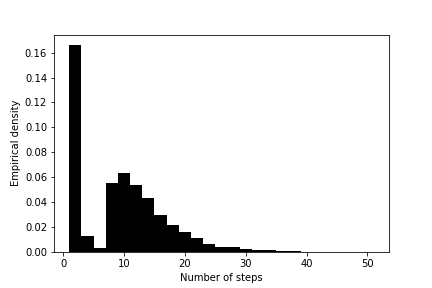
\includegraphics[width=0.7\linewidth, keepaspectratio]{duration_option_4rooms.png}
\decoRule
\caption{Empirical distribution of the duration of an option in the four rooms GridWorld, with mean $8.66$ steps. The $1$ step duration corresponds to cases when the agent unluckily goes in the wrong room from the starting hallway.}
\label{fig:duration}
\end{figure}

In that concrete example, the bound should be the same as for classical QL, as $\tau_{min} = 1$.

However, this bound can seem rather crude: $\tau$ could very well have an expectation of $100$ while $\tau_{\min} = 0.1$, in which case one can expect the theoretical result to be loose compared to reality. For that reason, a next step is to look more precisely at the proof in order to maybe get a tighter $\tilde T$, probably under some assumptions on $\tau$. For instance, the proof of Lemma \ref{lem:1b} uses Hoeffding's Inequality by bounding $\gamma_{t_k+1} \mathbf{P}_{t_k+1}(s,a) - \tilde{\mathbf{P}}(s,a)$ with $\gamma^{\tau_{min}}$, as for the uniform distribution; yet one can expect to get a better inequality, as this quantity should concentrate better in many cases.

Another interesting follow-up would be to adapt the proof to the more specific case of options.

Finally, the reader might have noticed that the bound holds for the sample complexity \emph{with respect to decision epochs} $t$, rather than the total duration time $\sigma_t$; yet, the latter one would make more sense, as the real cost is the learning time rather than the number of decisions made. This is another prospect to explore.
